
\section{Test}

\begin{figure}[h]
	\centering
	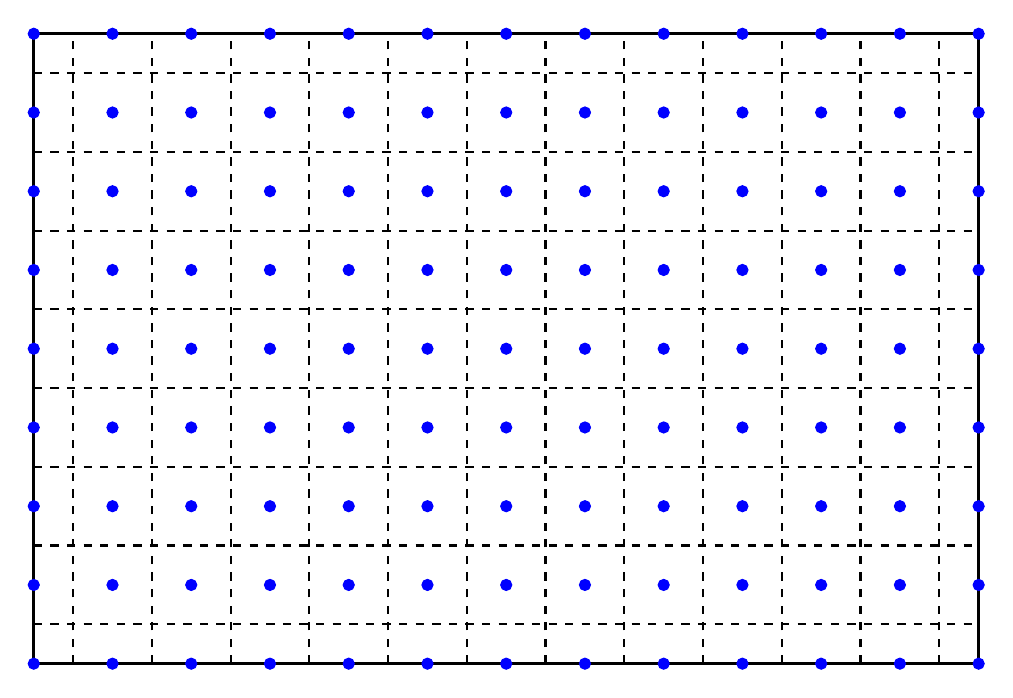
\begin{tikzpicture}
		\def\lx{12}
		\def\ly{8}
		\def\nx{13}
		\def\ny{9}
		\def\stepx{\lx/(\nx-1)}
		\def\stepy{\ly/(\ny-1)}
		\draw[very thick] (0,0) rectangle (\lx,\ly);
		% Nodes
		\foreach \x in {0,...,12}
		\foreach \y in {0,...,8}
		\filldraw[blue] ({\x*\stepx},{\y*\stepy}) circle (2pt);
		% Control volumes
		\foreach \x in {1,...,12}
		\draw[thick, dashed] ({-0.5*\stepx+\x*\stepx},0) -- ++(0,\ly);
		\foreach \y in {1,...,8}
		\draw[thick, dashed] (0,{-0.5*\stepy+\y*\stepy}) -- ++(\lx,0);
	\end{tikzpicture}
\end{figure}

\begin{figure}[h]
	\centering
	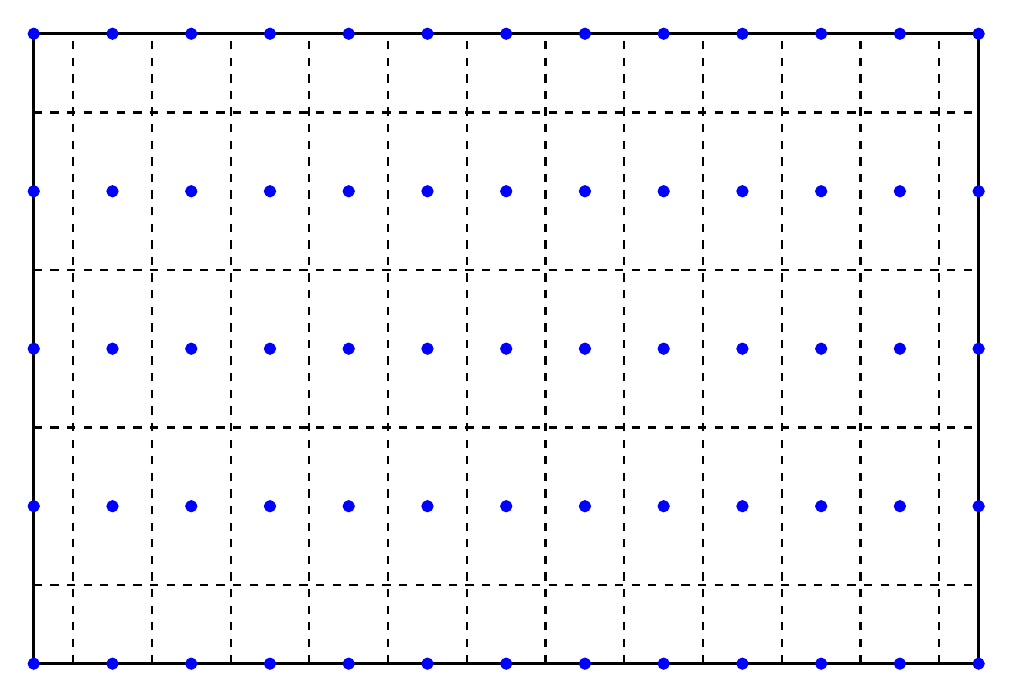
\begin{tikzpicture}
		\def\lx{12}
		\def\ly{8}
		\def\nx{13}
		\def\ny{5}
		\def\stepx{\lx/(\nx-1)}
		\def\stepy{\ly/(\ny-1)}
		\draw[very thick] (0,0) rectangle (\lx,\ly);
		% Nodes
		\foreach \x in {0,...,12}
		\foreach \y in {0,...,4}
		\filldraw[blue] ({\x*\stepx},{\y*\stepy}) circle (2pt);
		% Control volumes
		\foreach \x in {1,...,12}
		\draw[thick, dashed] ({-0.5*\stepx+\x*\stepx},0) -- ++(0,\ly);
		\foreach \y in {1,...,4}
		\draw[thick, dashed] (0,{-0.5*\stepy+\y*\stepy}) -- ++(\lx,0);
	\end{tikzpicture}
\end{figure}
